%------------------
% General Settings
%------------------
\def \docTitle      {User Manual}
\def \docSubTitle   {SMC2242/SMC4242}
\def \productNumber {SMCx242}
\def \productName   {Stepper Motor Controller}
\def \docAuthor     {LK-Instruments}
\def \docSubject    {\docAuthor \docTitle \docSubTitle}
\def \docKeywords   {LK-Instruments, Stepper Motor Controller, SMC2242, SMC4242}

\documentclass[a4paper, final, 12pt, oneside]{scrartcl}

%----------
% Packages
%----------
\usepackage{etex}
\reserveinserts{30}
\usepackage[utf8]{inputenc}
%\usepackage[latin1]{inputenc} % erlaubt Umlaute in der tex-Datei

\usepackage{slantsc}
\usepackage[urw-garamond]{mathdesign}
\usepackage{garamondx}
\usepackage[T1]{fontenc}

\usepackage[english]{babel}              % For the hyphenations in different languages
\usepackage[intlimits]{amsmath}          % math symbols
\usepackage{braket}                      % Dirac braket notation
\usepackage{graphicx}                    % include pictures
\usepackage{color}
\usepackage[shell]{gnuplottex}           % gnuplot in latex
\usepackage{pstricks}                    % post script tricks
\usepackage{listings}                    % enter programming code
\usepackage{fancyhdr}                    % make quite nice header/footer
\usepackage[version=3]{mhchem}           % chemistry stuff
\usepackage{relsize}
\usepackage{afterpage}
\usepackage{gensymb}
\usepackage{textcomp}

\usepackage{pgfplots}
\usepackage{tikz}                        % beautiful plots
\pgfplotsset{compat = newest}
\usepackage{units}                       % easy to use number-unit-package
\usepackage[section]{placeins}           % Float barrier for sections.

\usepackage{lcd}						             % Character LCD

\usetikzlibrary{shapes.geometric, arrows}	% Flow chart

\usepackage{listings}					% erlaubt Quellcode mit Zeilenumbr�chen

%----------------
% PDF properties
%----------------
\usepackage[
  pdftitle={\docAuthor~\docSubTitle~\docTitle}
 ,pdfsubject={\docSubject}
 ,pdfauthor={\docAuthor}
 ,pdfkeywords={\docKeywords}
 ,pdfcreator={\docAuthor}
 ,pdfstartview=Fit                       % startseite ganz anzeigen
 ,pdfborder={0 0 0}                      % links ohne umrandungen
 ,pdfdisplaydoctitle=true                % pdftitle statt dateinamen anzeigen
 ,pdfcenterwindow=true                   % position pdf in center of the screen
 ,setpagesize=true
]{hyperref}

%-------------------
% Header und Footer
%-------------------
\pagestyle{fancy}
\fancyhf{}        % clear all header/footer
\renewcommand{\headrulewidth}{0pt}
\renewcommand{\sectionmark}[1]{\markboth{#1}{}}
\renewcommand{\subsectionmark}[1]{\markright{#1}}
\fancyhead[LE,RO]{\textbf{\thepage}}
\fancyhead[CE]{\footnotesize{\textit{\nouppercase{\rightmark}}}}
\fancyhead[CO]{\footnotesize{\scshape{\nouppercase{\leftmark}}}}

% number equations with sections before equation-index
\numberwithin{equation}{section}
\numberwithin{table}{section}
\numberwithin{figure}{section}

%---------------------
% My code definitions
%---------------------

\newtheorem{envdefinition}{Definition}[section]
\newtheorem{envsatz}{Satz}

% special numbers and letters
\renewcommand{\i}{\mathrm{i}}                  % complex i
\newcommand{\e}{\mathrm{e}}                    % Eulers number
\renewcommand{\phi}{\varphi}                   % nicer phi
\renewcommand{\epsilon}{\varepsilon}           % nicer epsilon
\renewcommand{\theta}{\vartheta}               % nicer theta
\renewcommand{\rho}{\varrho}                   % nicer rho
%\newcommand{\degree}{^{\circ}}                 % degree-circle

% vectors and matrices
\renewcommand{\vec}[1]{\boldsymbol{#1}}
\newcommand{\Vek}[3]{\left(\begin{array}{c}#1\\#2 
\ifthenelse{\equal{#3}{}}{}{\\#3}\end{array}\right)}

% integral and derivative stuff:
\renewcommand{\d}[1]{\;\mathrm{d}#1}           % integeration d
% total derivative
\newcommand{\td}[1]{\frac{\mathrm{d}}{\mathrm{d}#1}\,}
\newcommand{\pd}[1]{\partial_{#1}\,}             % partial derivative

% Braket notation
\renewcommand{\bra}{\Bra}
\renewcommand{\ket}{\Ket}
\renewcommand{\braket}{\Braket}
\renewcommand{\set}{\Set}

% plus-minus with braces
\newcommand{\PM}{\ensuremath{\substack{+\\[-0.25em]-}\,}}
\renewcommand{\pm}{\PM}
\newcommand{\pmp}{\ensuremath{\substack{\mathsmaller{(}+\mathsmaller{)}\\[-0.25em]-}\,}}
\newcommand{\pmm}{\ensuremath{\substack{+\\[-0.25em]\mathsmaller{(}-\mathsmaller{)}}\,}}

%---------------------
% LCD
%---------------------

\definecolor{lightgrey}{rgb}{0.9,0.9,0.9}
\definecolor{darkgrey}{rgb}{0.2,0.2,0.2}
\definecolor{black}{rgb}{0,0,0}

\LCDcolors{black}{lightgrey}


%----------------------------------------------------------
% let the party start
%----------------------------------------------------------
\begin{document}


\pagecolor{black}
.
\vspace{4cm}
\begin{center}
  
\includegraphics[width=0.6\textwidth]{../general/logo_white.pdf}
\end{center}

\vspace*{2cm}
\begin{center}
  {\color{white} \Huge\textbf{\textsf{\docTitle}}}
\end{center}

\vspace*{1cm}
\begin{center}
  {\color{white} \Huge\textbf{\textsf{\productName}}}
\end{center}

%\vspace*{0.5cm}
\begin{center}
  {\color{white} \Huge\textbf{\textsf{\docSubTitle}}}
\end{center}

\afterpage{\nopagecolor}
\newpage


\thispagestyle{empty}
\section*{Notices}
\textcopyright~\docAuthor~2016.
No part of this manual may be reproduced in any form or by any means
(including electronic storage and retrieval or translation into a
foreign language) without prior agreement and written consent from \docAuthor.

\subsection*{Edition}
\today

\subsection*{Warranty}
The material contained in this document is provided \glqq as is\grqq, and is subject to
being changed, without notice, in future editions. Further, to the maximum extent
permitted by applicable law, \docAuthor~disclaims all warranties, either express or
implied, with regard to this manual and any information contained herein,
including but not limited to the implied warranties of merchantability and fitness
for a particular purpose.

\docAuthor~ shall not be liable for errors or for incidental
or consequential damages in connection with the furnishing, use, or performance of
this document or of any information contained herein. Should \docAuthor~and
the user have a separate written agreement with warranty terms covering the material
in this document that conflict with these terms, the warranty terms in the
separate agreement shall control.

\subsection*{Technology Licenses}
The hardware and/or software described in this document are furnished under a
license and may be used or copied only in accordance with the terms of such license.

%\subsection*{Restricted Rights Legend}
%If software is for use in the performance of a U.S. Government prime contract or
%subcontract, Software is delivered and licensed as “Commercial computer software”
%as defined in DFAR 252.227-7014 (June 1995), or as a “commercial item” as defined
%in FAR 2.101(a) or as “Restricted computer software” as defined in FAR 52.227-19
%(June 1987) or any equivalent agency regulation or contract clause. Use,
%duplication or disclosure of Software is subject to BitifEye’s standard commercial
%license terms, and non-DOD Departments and Agencies of the U.S. Government will
%receive no greater than Restricted Rights as defined in FAR 52.227-19(c)(1-2)
%(June 1987). U.S. Government users will receive no greater than Limited Rights as
%defined in FAR 52.227-14 (June 1987) or DFAR 252.227-7015 (b)(2) (November 1995),
%as applicable in any technical data.

%\subsection*{Safety Notices}


%\subsection*{Product Labels}
%\begin{itemize}
%  \item[\CE{cerm scaled \magstep5}] This electronic product is in compliance
%                                    with the EMC and Safety regulations of
%                                    the European Community.
%\end{itemize}



\newpage

\section{Technical Assistance}
If you need product assistance or if you have suggestions, contact \docAuthor.
You will find the contact information on the \docAuthor~homepage at
\begin{center}
  \url{http://www.lk-instruments.com}
\end{center}
Representatives of \docAuthor~are available during standard German business hours.
Before you contact \docAuthor, please note the actions you took before you experienced
the problem. Then describe those actions and the problem to the technical support
engineer.

\subsection{Found a mistake?}
We encourage comments about this publication. Please report any mistakes
to \docAuthor:
\begin{center}
  \href{mailto:support@lk-instruments.com}{\nolinkurl{support@lk-instruments.com}}
\end{center}






\newpage

\pagenumbering{roman}   % small roman page numbering
\tableofcontents
\newpage
\pagenumbering{arabic}  % now arabic page numbering
                        % for the rest of the document

Thank you for purchasing the \productNumber ~\productName. This user manual will explain you how to operate the \productName. Please take some time to read it carefully before operating the device. Keep the instructions in a safe place for future reference.

\section{Before you start}
\subsection{Package content}
Please check that the package contains all the following items:
\begin{itemize}
\item \productNumber ~\productName
\item Power supply cable
\item USB cable
\item User Manual
\end{itemize}

\subsection{Installing the device}
The \productName ~is designed for the inside use. Therefore it should not be used outside and kept away from water and moisture. Do not operate the unit near any heat sources or in direct sun light. When installing the device ensure to put it on a flat and leveled surface. Also ensure that there is adequate space around the device for ventilation.\\
After moving the unit to a different location, condensation inside the unit may occur. In this case please wait for some hours before you connect the \productName ~to the power supply.\\
Connect the device only to power sources that meet the specifications written on its rear panel.






\newpage
\section{General Information}
The \productNumber ~\productName ~is a universal controller for  bipolar stepper motors. It can be used to drive two (SMC2242) or four (SMC4242) stepper motors. There are three different firmware version available SMCx242-R for rotary axis, SMCx242-L for linear motion and SMCx242-U which features both options.


\begin{figure}[h]
\begin{center}
%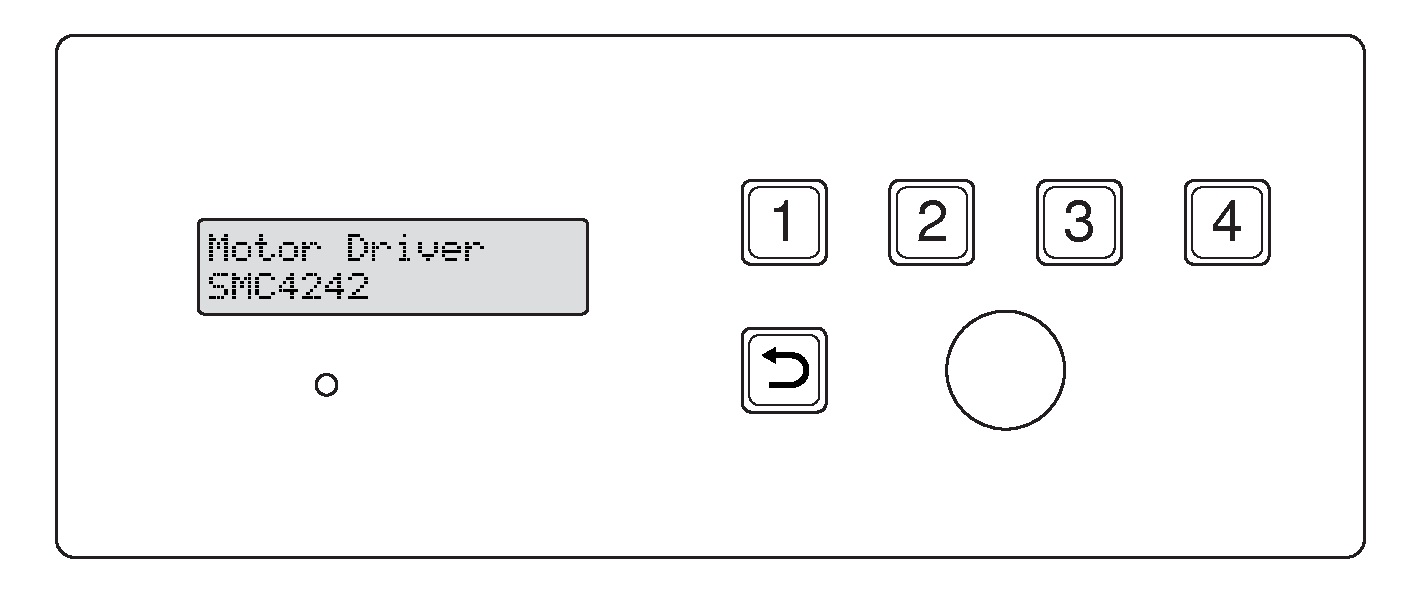
\includegraphics[width=12cm]{grafiken/SMCxxx2-0006_3_daub.pdf}
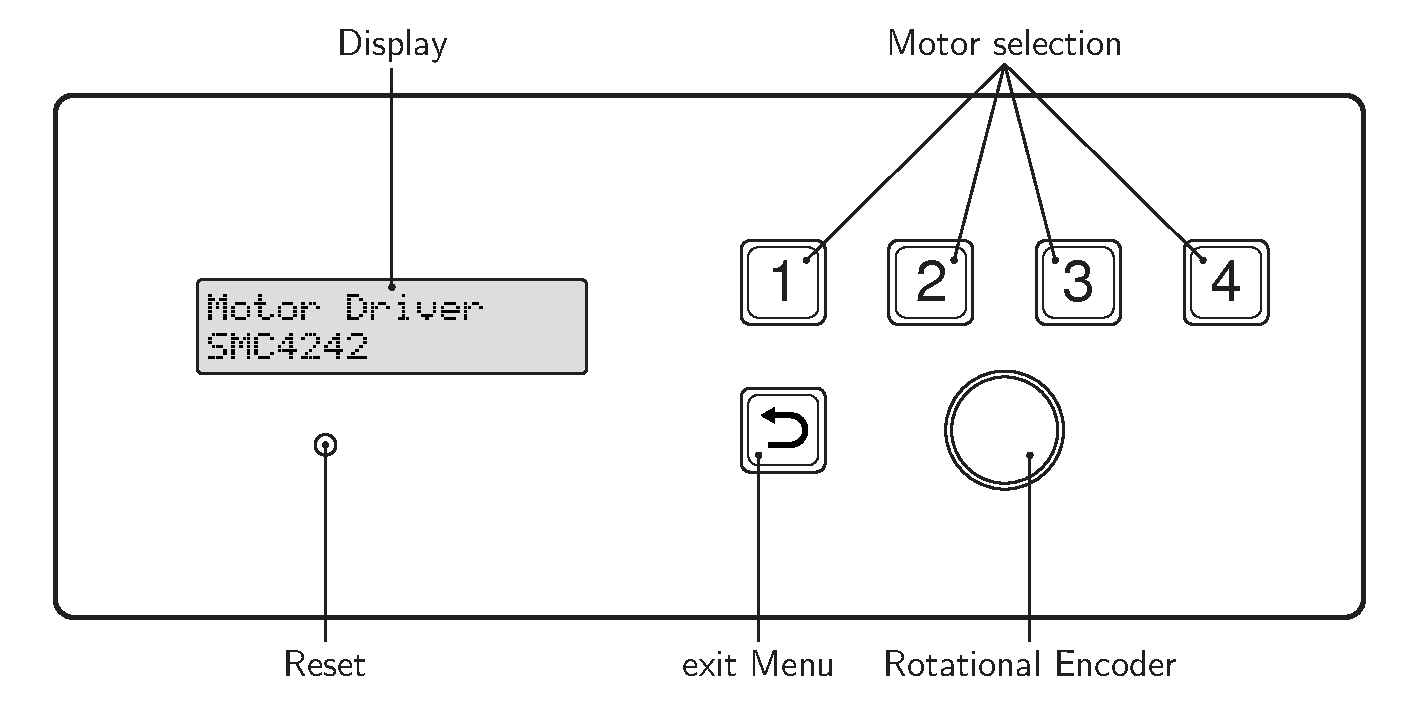
\includegraphics[width=12cm]{grafiken/SMCxxx2-0006_3_daub_text.pdf}
\end{center}
\caption[Front view of the \productNumber ~\productName.]{Front view of the \productNumber ~\productName.}
\label{frontpanel}
\end{figure}






\newpage
\section{Manual Operation}
The \productNumber ~\productName ~features two operation modes. It can be either operated using the manual user interface or remote controlled by a computer. In this section the manual operation of the device is explained.
\subsection{Menu structure}
After turning on the \productName ~it comes up with its start screen. Turning the rotary encoder serves to scroll through the menus (see figure~\ref{main_menu}). Pressing the rotary encoder enters the selected menu. Pressing the menu-escape-button leaves the menu again.

\tikzstyle{menu_style} = [rectangle, rounded corners, minimum width=3cm, minimum height=1cm,text centered, draw=black]
\tikzstyle{arrow} = [thick,<->,>=latex]
\def \textWidth {7cm}

\begin{figure}[H]
\begin{tikzpicture}[node distance=2cm]
\node (start) [menu_style] {
\begin{minipage}[h]{5cm}
\LCD{2}{16}|Motor Driver|
|SMC4242|
\end{minipage}
 \hfill
\begin{minipage}[h]{\textWidth}
Start screen\\
Display firmware version.
\end{minipage}
};

\node (motor_pos) [menu_style, below of=start] {
\begin{minipage}[h]{5cm}
\LCD{2}{16}|Change motor|
|position|
\end{minipage}
 \hfill
\begin{minipage}[h]{\textWidth}
Menu: Change motor position\\
Position is displayed and can be changed.
\end{minipage}
};

\node (step_multiplier) [menu_style, below of=motor_pos] {
\begin{minipage}[h]{5cm}
\LCD{2}{16}|Set step|
|multiplier|
\end{minipage}
 \hfill
\begin{minipage}[h]{\textWidth}
Menu: Set step multiplier\\
Edit multiplier for rotary encoder.
\end{minipage}
};

\node (step_unit) [menu_style, below of=step_multiplier] {
\begin{minipage}[h]{5cm}
\LCD{2}{16}|Change step|
|unit|
\end{minipage}
 \hfill
\begin{minipage}[h]{\textWidth}
Menu: Change step unit\\
Define the displayed unit.
\end{minipage}
};

\node (optical_zero) [menu_style, below of=step_unit] {
\begin{minipage}[h]{5cm}
\LCD{2}{16}|Define optical|
|zero position|
\end{minipage}
 \hfill
\begin{minipage}[h]{\textWidth}
Menu: Define optical zero position\\
Edit the zero offset.
\end{minipage}
};

\node (internal_prog) [menu_style, below of=optical_zero] {
\begin{minipage}[h]{5cm}
\LCD{2}{16}|Run internal|
|program|
\end{minipage}
 \hfill
\begin{minipage}[h]{\textWidth}
Menu: Run internal program\\
Step through the program list.
\end{minipage}
};

\node (const_speed) [menu_style, below of=internal_prog] {
\begin{minipage}[h]{5cm}
\LCD{2}{16}|Set constant|
|angular speed|
\end{minipage}
 \hfill
\begin{minipage}[h]{\textWidth}
Menu: Set constant angular speed\\
Start/Stop continuous movement.
\end{minipage}
};

\node (step_wait_time) [menu_style, below of=const_speed] {
\begin{minipage}[h]{5cm}
\LCD{2}{16}|Change step|
|wait time|
\end{minipage}
 \hfill
\begin{minipage}[h]{\textWidth}
Menu: Change step wait time\\
Edit time between steps.
\end{minipage}
};

\node (substep) [menu_style, below of=step_wait_time] {
\begin{minipage}[h]{5cm}
\LCD{2}{16}|Change motor|
|substep|
\end{minipage}
 \hfill
\begin{minipage}[h]{\textWidth}
Menu: Change motor substep\\
Edit number of substeps.
\end{minipage}
};

%----------------------------------------------------------------------
% zusaetzliche Menues hier einfuegen!
%----------------------------------------------------------------------

\node (save) [menu_style, below of=substep] {
\begin{minipage}[h]{5cm}
\LCD{2}{16}|Save all current|
|configurations|
\end{minipage}
 \hfill
\begin{minipage}[h]{\textWidth}
Menu: Save all current configurations\\
Save configurations to EEPROM.
\end{minipage}
};

\node (load) [menu_style, below of=save] {
\begin{minipage}[h]{5cm}
\LCD{2}{16}|Load last|
|configuration|
\end{minipage}
 \hfill
\begin{minipage}[h]{\textWidth}
Menu: Load last configuration\\
Load configuration from EEPROM.
\end{minipage}
};

\node (zero_cal) [menu_style, below of=load] {
\begin{minipage}[h]{5cm}
\LCD{2}{16}|Run zero|
|calibration|
\end{minipage}
 \hfill
\begin{minipage}[h]{\textWidth}
Menu: Run zero calibration\\
Find mechanical zero position.
\end{minipage}
};

\draw [arrow] (start) -- (motor_pos);
\draw [arrow] (motor_pos) -- (step_multiplier);
\draw [arrow] (step_multiplier) -- (step_unit);
\draw [arrow] (step_unit) -- (optical_zero);
\draw [arrow] (optical_zero) -- (internal_prog);
\draw [arrow] (internal_prog) -- (const_speed);
\draw [arrow] (const_speed) -- (step_wait_time);
\draw [arrow] (step_wait_time) -- (substep);
%------------------------------------------
\draw [arrow] (substep) -- (save);
\draw [arrow] (save) -- (load);
\draw [arrow] (load) -- (zero_cal);
\draw [arrow] (zero_cal.east) -- +(1,0) |- (start.east);
\end{tikzpicture}
\caption[Overview of the available menus.]{Overview of the available menus. By rotating the rotary encoder one can navigate through the list of menus as indicated by the arrows.}
\label{main_menu}
\end{figure}

\subsubsection{Display structure}
In almost every menu four values are displayed. Depending on the previously selected menu the values correspond to different quantities. Where\\
the upper left value accompanies to Motor 0,\\
the upper right value accompanies to Motor 1,\\
the lower left value accompanies to Motor 2 and\\
the lower right value accompanies to Motor 3.

\subsubsection{Motor selection}
To select a motor there are four buttons. Motor selection can solely be done in an entered menu. To select a motor, press the respective motor-selection button. A selected motor is signed with an arrow on the display. Pressing the selection-button again deselects the motor. Once a motor is selected its appropriate value can be changed by turning the rotary encoder. By leaving a menu without motor deselection the selected motor(s) stay selected in an other menu.

\subsubsection{Start screen}
When entering the menu behind the start screen, the firmware version will be displayed.
\LCD{2}{16}||
|v1.3|

\subsubsection{Menu: Change motor position}
\label{menu_motor_pos}
In this menu the current motor positions are displayed and can be changed by the operator. The default display unit is degree. The position of a selected motor can be changed by turning the rotary encoder. Default steps for different units are:
\begin{itemize}
\item $1\degree$ if unit is degree
\item $0.125 \cdot \pi$ if unit is radian
\item 1 step if unit is steps
\end{itemize}

\LCD{2}{16}|{rarrow}0.0{pi}   {rarrow}0.0|
           |{rarrow}0st    {rarrow}0.0|

When pressing the rotary encoder in this menu one enters the fast moving mode. Pressing the rotary encoder again leaves the fast mode. The fast moving mode can be noticed by another marking arrow. Default steps in fast mode are:
\begin{itemize}
\item $10\degree$ if unit is degree
\item $0.125 \cdot \pi$ if unit is radian
\item 100 steps if unit is steps
\end{itemize}

\LCD{2}{16}|>0.0   >0.0||>0.0   >0.0|

\subsubsection{Menu: Set step multiplier}
In this menu one can adjust a step multiplier. The step multiplier is applied if the step unit is degree or radian. The standard value is 1.0. If the step multiplier differs from 1.0 the corresponding motor will rotate more or less steps with each rotation of the rotary encoder.\\
For example: if the step multiplier for motor 0 is 1.0 and the step multiplier for motor 2 is 4.0, motor 2 will move four times more steps than motor 0 when changing the motors positions. Negative values are allowed as well. This will result in counter direction movements.

\LCD{2}{16}|{rarrow}1.0x   {rarrow}-0.5x|
|{rarrow}2.0x    1.0x|

\subsubsection{Menu: Change step unit}
In this menu one can choose the unit of the displayed position. There are three possible choices for each motor:
\begin{itemize}
\item degree
\item radian
\item step
\end{itemize}

\LCD{2}{16}|{rarrow}radian {rarrow}degree|
|{rarrow}step    degree|

\subsubsection{Menu: Define optical zero position}
In this menu one can define the optical zero position. This is necessary due to a mostly unknown placement of the optical element mounted to the motor. Here one can once adjust the desired optical zero position manually. The optical zero position is always defined in steps. In this menu there is also a fast mode available (please refer to \ref{menu_motor_pos} for details about the fast mode). After adjustment it is recommended to save this configuration (see \ref{menu_save}).
When performing a zero calibration, as explained in \ref{menu_zero_cal}, the zero position will be the defined optical zero position.

\LCD{2}{16}|{rarrow}0st     0st|
| 0st     0st|

\subsubsection{Menu: Run internal program}
This menu allows the user to step through the internal program list. This function is available only if a program has previously been defined (see \ref{section_instruction_set}).

\LCD{2}{16}|Program running|
|Step 0|

\subsubsection{Menu: Set constant angular speed}
Here the motors can be set into an infinite moving state in clockwise (CW) or counter clockwise (CCW) direction. To get the motors moving with different velocities one needs to change the wait times between two steps (see \ref{menu_step_wait_time}).

\LCD{2}{16}|{rarrow}CW     {rarrow}CCW|
| STOP    STOP|

\subsubsection{Menu: Change step wait time}
\label{menu_step_wait_time}
Here the wait time between two steps can be changed. This results in faster or slower motor movements. The default value is 3 milliseconds. We do not recommend to use shorter wait times, even if this works.

\LCD{2}{16}|{rarrow}3 ms   {rarrow}3 ms|
|{rarrow}3 ms    3 ms|

\subsubsection{Menu: Change motor substeps}
In this menu one can change the motor substeps. Possible values are 1, 2, 4, 8, 16 or 32.

\LCD{2}{16}|{rarrow}1      {rarrow}2|
| 4      {rarrow}8|

%----------------------------------------------------------------------
% zusaetzliche Menues hier einfuegen!
%----------------------------------------------------------------------

\subsubsection{Menu: Save current configurations}
\label{menu_save}
To save the current \productName ~configurations enter this menu and turn the rotary encoder in any direction. The menu will be automatically leaved when saving is finished.\\
Note: The configurations for all motors will be saved.

\LCD{2}{16}|Save all current|
|configurations|

\subsubsection{Menu: Load last configuration}
To load the last saved \productName ~configurations enter this menu and turn the rotary encoder in any direction. The menu will be leaved automatically when loading has
finished.\\
Note: The last saved configuration is loaded automatically when powering on the \productName.\\
Note: There is just one memory space for a configuration.

\LCD{2}{16}|Load all saved|
|configurations|

\subsubsection{Menu: Run zero calibration}
\label{menu_zero_cal}
Here one can calibrate the motor zero position for each motor. To perform a zero calibration select the motors to be calibrated and turn the rotary encoder. Note, that during zero calibration no actions can be done on the device, even serial commands will not be accepted. The zero calibration will automatically deselect a motor when its calibration is finished. The zero calibration menu will be automatically leaved when calibration is finished.

\LCD{2}{16}|{rarrow}Mot 0  {rarrow}Mot 1|
| Mot 2   Mot 3|











\newpage

\section{Computer Control}
\subsection{Communication Settings}
In order to remote control the \productName ~from a computer, it needs to be connected to the computer via the USB cable. The \productName ~will show up as a new Virtual COM Port (VCP). In some cases it might be necessary to install some drivers. They can be found here:\\
\url{http://www.ftdichip.com/Drivers/VCP.htm}\\
Once the Virtual COM Port has been installed successfully, the \productName ~can be controlled by sending commands via a serial terminal. A list of all available commands can be found in section~\ref{section_instruction_set}. The serial terminal needs to be configured as follows:
\begin{itemize}
\item 57600 Baud
\item 8 bit character size
\item no parity bit
\item 1 stop bit
\item no flow control
\end{itemize}

\subsection{Instruction set}
\label{section_instruction_set}
\lstMakeShortInline[language=sh,basicstyle=\ttfamily]@

The \productName ~has the following commands which can be used. Note, that the command parser is case sensitive. The command parameters, denoted by @<xxx>@, must be separated by either @SPACE@ or ``,'' or ``;'' or @TAB@. The command is completed by sending a  Carriage Return + Line Feed (@CRLF@) or Line Feed (@LF@).
\def \vdistace {3ex}
\vspace{\vdistace}

\begin{tabular}{ll}
Command: & @*RST@\\
Function: & Resets the \productName ~to the initial state.\\
Example: & @*RST@
\end{tabular}

\vspace{\vdistace}

\begin{tabular}{ll}
Command: & @*IDN?@\\
Function: & Returnes the identification name of the \productName.\\
Example: & @*IDN?@
\end{tabular}

\vspace{\vdistace}

\begin{tabular}{ll}
Command: & @*IDN <driver_idn>@\\
Function: & Sets the identification of the \productName.\\
Note: & The maximum number of characters is 20.\\
Example: & @*IDN NewName@\\
		& Sets the string ``NewName'' as IDN.
\end{tabular}

\vspace{\vdistace}

\begin{tabular}{ll}
Command: & @GETMOTSTATE <mot>@\\
Function: & Returns whether motor @<mot>@ is turned on or off.\\
Example: & @GETMOTSTATE 3@\\
		& Returns 1 if motor 3 is turned on or 0 if motor 3 is turned off.
\end{tabular}

\vspace{\vdistace}

\begin{tabular}{ll}
Command: & @MOVEABS <mot> <pos> <unit>@\\
Function: & Moves motor @<mot>@ to the absolute position @<pos> <unit>@.\\
		& The units can be steps, degree or radians.\\
Note: & The units must be written in lower case letters.\\
Example: & @MOVEABS 0 0 deg@\\
		& @MOVEABS 0 0 pi@\\
		& @MOVEABS 0 0 steps@\\
		& The examples do the same in different units.
\end{tabular}

\vspace{\vdistace}

\begin{tabular}{ll}
Command: & @MOVEREL <mot> <pos> <unit>@\\
Function: & Moves motor @<mot>@ relative to the current position.\\
		& The units can be steps, degree or radians.\\
Note: & The units must be written in lower case letters.\\
Example: & @MOVEREL 2 22.5 deg@\\
		& @MOVEREL 2 0.125 pi@\\
		& Both examples do the same in different units.
\end{tabular}

\vspace{\vdistace}

\begin{tabular}{ll}
Command: & @ZERORUN <mot>@\\
Function: & Finds the mechanical zero position of the motor.\\
Note: & During motor zero run no communication or usage\\
		& of the \productName ~is allowed.\\
Example: & @ZERORUN 1@\\
		& Finds the mechanical zero position of motor 1.
\end{tabular}

\vspace{\vdistace}

\begin{tabular}{ll}
Command: & @ENABLE <mot> <on/off>@\\
Function: & Turns motor @<mot>@ on (1) or off (0).\\
Note: & Both for enabeling and disabeling of a motor the same command is used.\\
Example: & @ENABLE 2 1@\\
		& Turns motor 2 on.\\
		& @ENABLE 2 0@\\
		& Turns motor 2 off.
\end{tabular}

\vspace{\vdistace}

\begin{tabular}{ll}
Command: & @GETPOS <mot> <unit>@\\
Function: & Returns the actual motor position in the given unit.\\
Example: & @GETPOS 1 deg@\\
		& Returns the current position of motor 1 in degree.
\end{tabular}

\vspace{\vdistace}

\begin{tabular}{ll}
Command: & @SAVECONF@\\
Function: & Saves all current configurations for all motors.\\
Note: & The driver configuration is stored in an EEPROM.\\
		& Maximum write cycles are 100000.\\
Example: & @SAVECONF@
\end{tabular}

\vspace{\vdistace}

\begin{tabular}{ll}
Command: & @LOADCONF@\\
Function: & Loads all saved configurations for all motors.\\
Example: & @LOADCONF@\\
\end{tabular}

\vspace{\vdistace}

\begin{tabular}{ll}
Command: & @GETOPTZEROPOS <mot>@\\
Function: & Returns the optical zero position of motor @<mot>@.\\
Example: & @GETOPTZEROPOS 3@\\
		& Returns the optical zero position of motor 3.
\end{tabular}

\vspace{\vdistace}

\begin{tabular}{ll}
Command: & @SETOPTZEROPOS <mot>@\\
Function: & Set the optical zero position for motor @<mot>@.\\
Note: & For the optical zero position the unit is always steps.\\
Example: & @SETOPTZEROPOS 3 574@\\
		& Sets the optical zero position of motor 3 to 574 steps.
\end{tabular}

\vspace{\vdistace}

\begin{tabular}{ll}
Command: & @GETWAITTIME <mot>@\\
Function: & Returns the wait time between two steps of a motor.\\
Example: & @GETWAITTIME 0@\\
		& Returns the wait time between two steps of motor 0.
\end{tabular}

\vspace{\vdistace}

\begin{tabular}{ll}
Command: & @SETWAITTIME <mot> <time>@\\
Function: & Sets the wait time between two steps to @<time>@ milliseconds\\
		& for motor @<mot>@.\\
Note: & The wait time must be an integer. The unit for the wait time\\
		& is always milliseconds.\\
Example: & @SETWAITTIME 1 5@\\
		& Sets the wait time of motor 1 to 5 milliseconds.
\end{tabular}

\vspace{\vdistace}

\begin{tabular}{ll}
Command: & @STOPALL@\\
Function: & Stops all motor movements immediately.\\
Example: & @STOPALL@\\
\end{tabular}

\vspace{\vdistace}

\begin{tabular}{ll}
Command: & @FACTORYRESET@\\
Function: & Resets the \productName ~to factory state.\\
Example: & @FACTORYRESET@\\
\end{tabular}

\vspace{\vdistace}

\begin{tabular}{ll}
Command: & @ISMOVING <mot>@\\
Function: & Returns the motor moving state.\\
		& 1: motor @<mot>@ is moving.\\
		& 0: motor @<mot>@ doesn't move.\\
Example: & @ISMOVING 0@\\
\end{tabular}

\vspace{\vdistace}

\begin{tabular}{ll}
Command: & @SETCONSTSPEED <mot> <dir> <time>@\\
Function: & Enables motor @<mot>@ to move infinite in direction @<dir>@. Possible\\
		& values for @<dir>@ are clock wise @CW@ or counter clock wise @CCW@.\\
		& @<time>@ specifies the time for one full rotation.\\
Example: & @SETCONSTSPEED 1 CW 10.0@\\
		& Moves motor 1 infinite in clockwise direction.\\
		& One full rotation takes 10 seconds.
\end{tabular}

\vspace{\vdistace}

\begin{tabular}{ll}
Command: & @SETFORBZONE <mot> <start> <stop>@\\
Function: & Defines a forbidden zone for motor @<mot>@. The motor will not move\\
		& into this zone. @<start>@ must be always smaller than @<stop>@. The unit\\
		& for @<start>@ and @<stop>@ is always steps.\\
Example: & @SETFORBZONE 0 148 1333@\\
		& Defines a forbidden zone for motor 0 between step 148 and step 1333.
\end{tabular}

\vspace{\vdistace}

\begin{tabular}{ll}
Command: & @ENABFORBZONE <mot> <val>@\\
Function: & Enables @<val=1>@ or disables @<val=0>@ the defined forbidden zone\\
		& for motor @<mot>@\\
Example: & @ENABFORBZONE 0 1@\\
		& Enables the forbidden zone for motor 0.\\
		& @ENABFORBZONE 3 0@\\
		& Disables the forbidden zone for motor 3.
\end{tabular}

\vspace{\vdistace}

\begin{tabular}{ll}
Command: & @SETPROGSTEP <step> <posMot0> <posMot1> <posMot2> <posMot3> <mode>@\\
Function: & Defines an internal program step for all four motors. @<step>@ is the program\\
		& sequence number. The position of all motors @<posMot0...4>@ must be given\\
		& in steps. The mode defines if the movement is to an absolute position @<mode=ABS>@\\
		& or if the movement is relative to the current motor position @<mode=REL>@.\\
Example: & @SETPROGSTEP 0 112 294 0 12 ABS@\\
		& Defines the internal program step 0 so that motor 0 moves to step 112,\\
		& motor 1 moves to step 294, motor 2 moves to step 0 and motor 3 moves to step 12.\\
		& @SETPROGSTEP 1 10 10 -10 -10 REL@\\
		& Defines the internal program step 1 so that motor 0 and motor 1 move\\
		& 10 steps forward relative to the actual position and motor 2 and 3 move\\
		& 10 steps backwards from the actual position.
\end{tabular}

\lstDeleteShortInline@

\newpage


\section{Specifications}


\begin{table}[htbp]
\label{motor_specs}
\caption[Specifications of supported motors.]{Specifications of supported motors.}
\centering
\begin{tabular}{|l|c|c|}
\hline 
 & SMC2242 & SMC4242 \\ \hline 
Number of Motors: & 2 & 4 \\ \hline
Motor Type: & \multicolumn{2}{c|}{Bipolar Stepper Motor} \\ \hline
Motor Drive Voltage: & \multicolumn{2}{c|}{\unit[24]{V}} \\ \hline
Motor Current: & \multicolumn{2}{c|}{up to \unit[2.5]{A} peak or \unit[1.75]{A} RMS} \\ \hline
\end{tabular}
\end{table}


\begin{table}[htbp]
\label{features_of_versions}
\caption[Features of different versions.]{Features of different versions.}
\centering
\begin{tabular}{|l|c|c|c|}
\hline 
 & SMCx242-R & SMCx242-L & SMCx242-U \\ \hline 
Units: & $\degree$, $\pi$, steps & m, cm, mm, steps & $\degree$, $\pi$, m, cm, mm, steps, user-defined \\ \hline
Substeps: & \multicolumn{3}{c|}{1, 2, 4, 8, 16, 32} \\ \hline
Steps per Revolution: & \multicolumn{3}{c|}{200, 400} \\ \hline
Gear Ratio: & \multicolumn{3}{c|}{???} \\ \hline
Reference/Limit Switches: & 1 & \multicolumn{2}{c|}{3} \\ \hline
\end{tabular}
\end{table}


\begin{table}[htbp]
\label{motor_specs}
\caption[Technical Specifications.]{Technical Specifications.}
\centering
\begin{tabular}{|l|c|}
\hline 
Power requirements: & ? \\ \hline 
Power consumption: & \unit[]{W} \\ \hline 
Dimensions: & \unit[245]{mm} (W) x \unit[85]{mm} (H) x \unit[260]{mm} (D) \\ \hline 
Weight (without package): & \unit[]{kg} \\ \hline 
\end{tabular}
\end{table}



\section{Pinout}
The connectors for for the stepper motors are 9-Pin D-Type, female connectors. Please refer to figure~\ref{pin_out} for their pinout.

\begin{figure}[h]
\begin{center}
\begin{minipage}[h]{5cm}
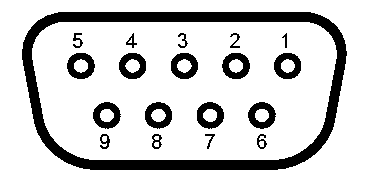
\includegraphics[width=5cm]{grafiken/Numbered_DE9_female_Diagram.pdf}
\end{minipage}
\hspace{1cm}
\begin{minipage}[h]{5cm}
\begin{tabular}{|c|c|}
\hline 
\textbf{Pin} & \textbf{Description} \\ \hline 
1 & Bridge B output 1 \\ \hline 
2 & Bridge B output 2 \\ \hline 
3 & Bridge A output 2 \\ \hline 
4 & Bridge A output 1 \\ \hline 
5 & Ground \\ \hline 
6 & \unit[+5]{V} \\ \hline 
7 & Reference/Limit Switch 1 \\ \hline 
8 & Reference/Limit Switch 2 \\ \hline 
9 & Reference/Limit Switch 3 \\ \hline 
\end{tabular}
\end{minipage}
\end{center}
\caption[Pinout of the Motor Connector.]{Pinout of the Motor Connector.}
\label{pin_out}
\end{figure}










\newpage


\end{document}
